\section{Computer Networks and the Internet}

\subsection{Network Edge}
\key{Network edge} Applications and hosts

\subsection{Network Core}
\key{Network core} Routers, Network of networks

\key{Internet protocol stack}
\begin{figure}[H]
  \centering
  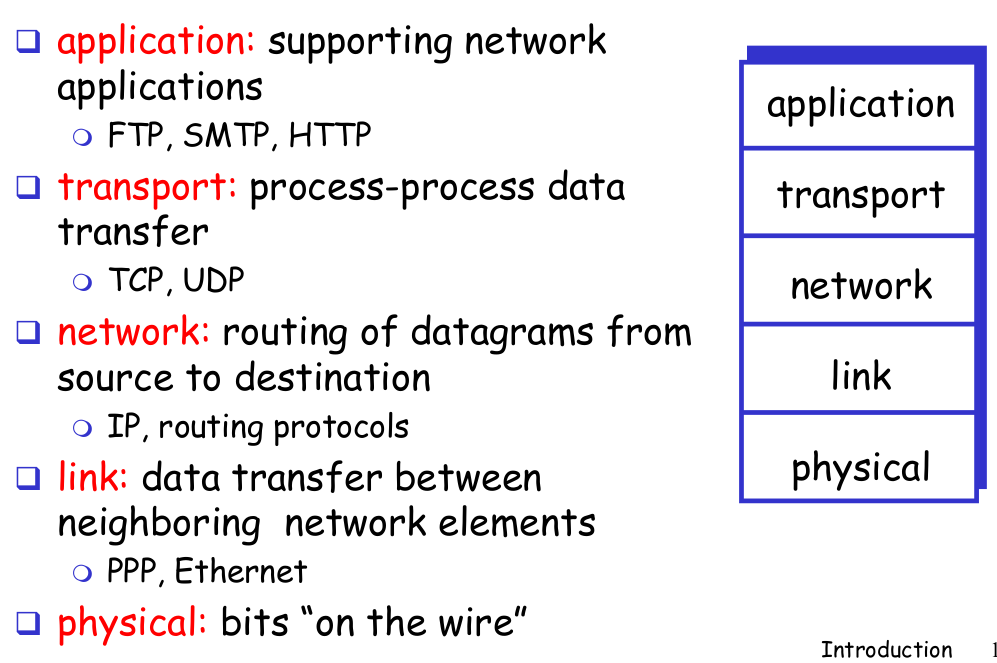
\includegraphics[width=0.5\textwidth]{stack}
\end{figure}

\key{Apps Using TCP} HTTP (Web), FTP (file transfer), Telnet (remote login), SMTP (email)

\key{Apps using UDP} streaming media, teleconferencing, \textbf{DNS}, Internet telephony

\subsection{Delay \& loss in packet-switched networks}

\key{Four sources of delay}
\begin{enumerate}
  \item Transmission delay $d_{\text{trans}}$
  \item Propagation delay $d_{\text{prop}}$
  \item Nodal processing $d_{\text{proc}}$
  \item Queueing $d_{\text{queue}}$
\end{enumerate}
\begin{figure}[H]
  \centering
  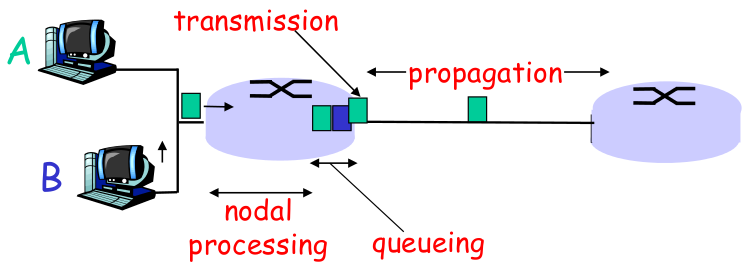
\includegraphics[width=0.5\textwidth]{delay}
\end{figure}

\key{Virtual Circuit} With VC, two packets with the same destination can be assigned two different
VC\# and forced to take different paths.
